% Created by tikzDevice version 0.11 on 2018-05-04 09:33:42
% !TEX encoding = UTF-8 Unicode
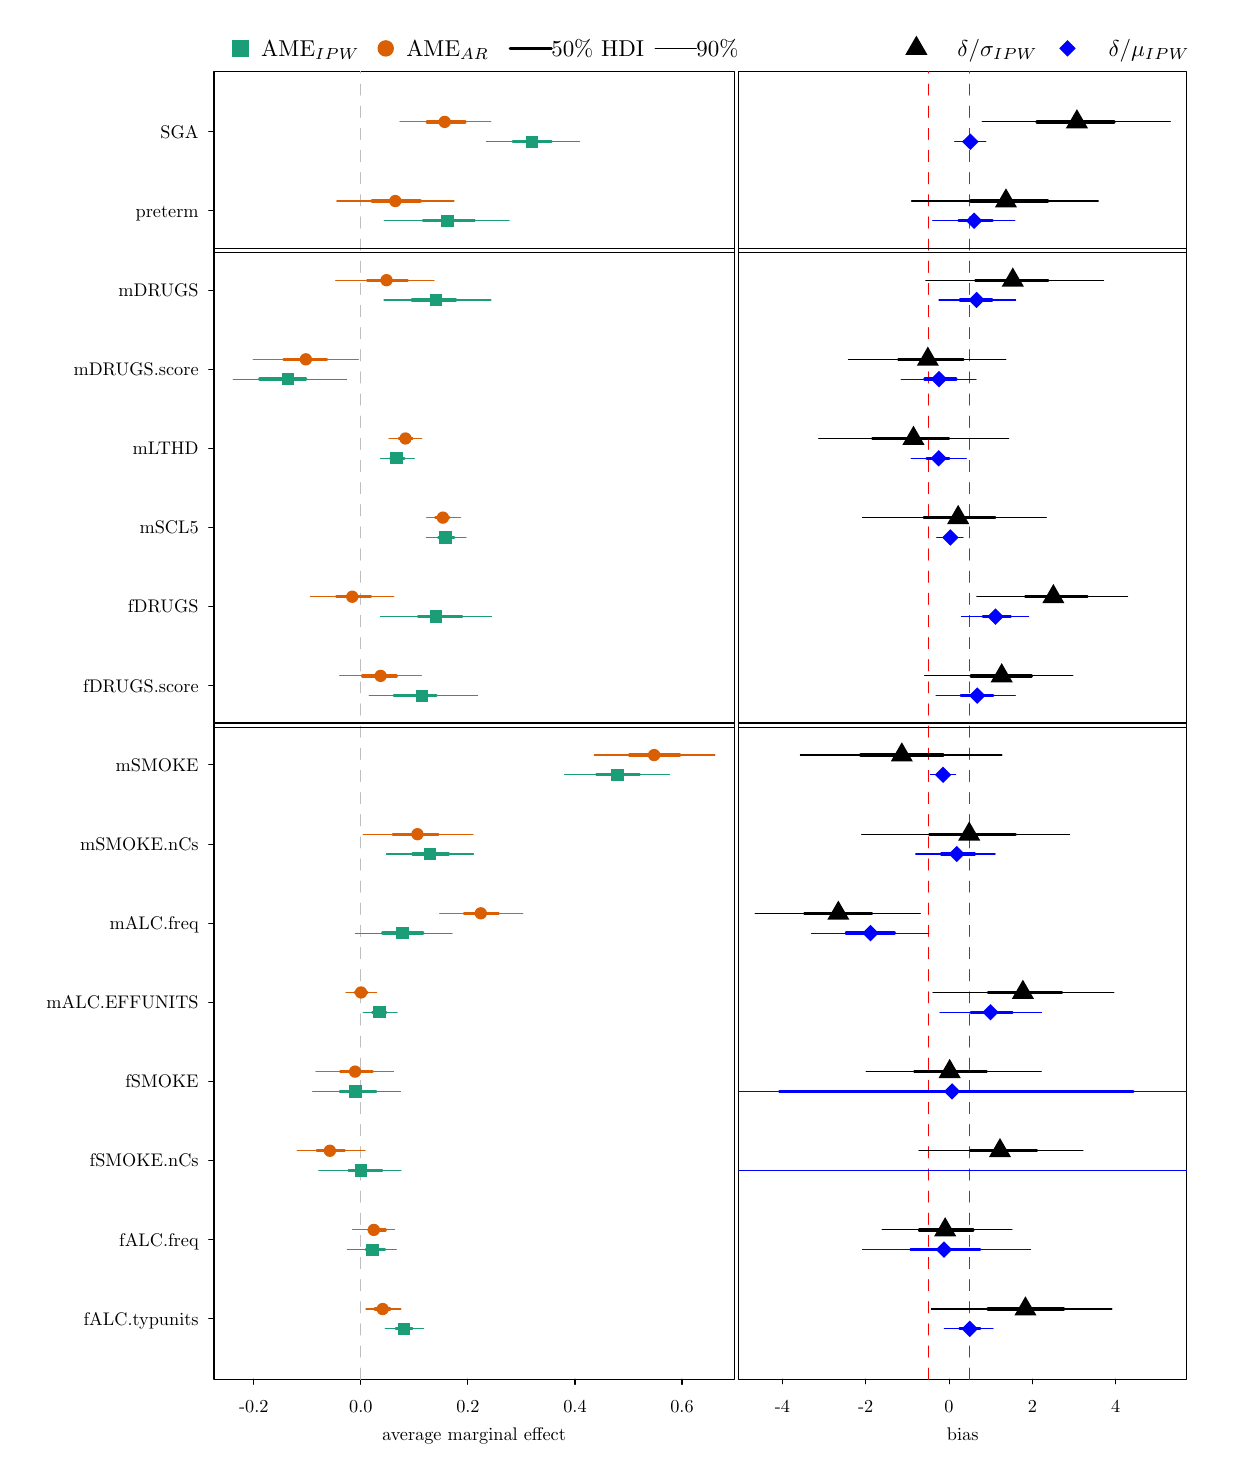
\begin{tikzpicture}[x=1pt,y=1pt]
\definecolor{fillColor}{RGB}{255,255,255}
\path[use as bounding box,fill=fillColor,fill opacity=0.00] (0,0) rectangle (426.79,512.15);
\begin{scope}
\path[clip] (  0.00,  0.00) rectangle (426.79,512.15);
\definecolor{drawColor}{RGB}{0,0,0}

\path[draw=drawColor,line width= 0.4pt,line join=round,line cap=round] ( 81.73, 23.76) -- (236.45, 23.76);

\path[draw=drawColor,line width= 0.4pt,line join=round,line cap=round] ( 81.73, 23.76) -- ( 81.73, 21.88);

\path[draw=drawColor,line width= 0.4pt,line join=round,line cap=round] (120.41, 23.76) -- (120.41, 21.88);

\path[draw=drawColor,line width= 0.4pt,line join=round,line cap=round] (159.09, 23.76) -- (159.09, 21.88);

\path[draw=drawColor,line width= 0.4pt,line join=round,line cap=round] (197.77, 23.76) -- (197.77, 21.88);

\path[draw=drawColor,line width= 0.4pt,line join=round,line cap=round] (236.45, 23.76) -- (236.45, 21.88);

\node[text=drawColor,anchor=base,inner sep=0pt, outer sep=0pt, scale=  0.66] at ( 81.73, 11.88) {-0.2};

\node[text=drawColor,anchor=base,inner sep=0pt, outer sep=0pt, scale=  0.66] at (120.41, 11.88) {0.0};

\node[text=drawColor,anchor=base,inner sep=0pt, outer sep=0pt, scale=  0.66] at (159.09, 11.88) {0.2};

\node[text=drawColor,anchor=base,inner sep=0pt, outer sep=0pt, scale=  0.66] at (197.77, 11.88) {0.4};

\node[text=drawColor,anchor=base,inner sep=0pt, outer sep=0pt, scale=  0.66] at (236.45, 11.88) {0.6};

\path[draw=drawColor,line width= 0.4pt,line join=round,line cap=round] ( 67.32, 23.76) --
	(255.28, 23.76) --
	(255.28,496.31) --
	( 67.32,496.31) --
	( 67.32, 23.76);
\end{scope}
\begin{scope}
\path[clip] (  0.00,  0.00) rectangle (256.07,512.15);
\definecolor{drawColor}{RGB}{0,0,0}

\node[text=drawColor,anchor=base,inner sep=0pt, outer sep=0pt, scale=  0.66] at (161.30,  1.58) {average marginal effect};
\end{scope}
\begin{scope}
\path[clip] ( 67.32, 23.76) rectangle (255.28,496.31);
\definecolor{drawColor}{RGB}{190,190,190}

\path[draw=drawColor,line width= 0.4pt,dash pattern=on 4pt off 4pt ,line join=round,line cap=round] (120.41, 23.76) -- (120.41,496.31);
\definecolor{fillColor}{RGB}{27,158,119}

\path[fill=fillColor] (180.11,468.72) --
	(184.57,468.72) --
	(184.57,473.17) --
	(180.11,473.17) --
	cycle;

\path[fill=fillColor] (149.45,440.12) --
	(153.90,440.12) --
	(153.90,444.57) --
	(149.45,444.57) --
	cycle;

\path[fill=fillColor] (145.38,411.52) --
	(149.84,411.52) --
	(149.84,415.98) --
	(145.38,415.98) --
	cycle;

\path[fill=fillColor] ( 91.94,382.92) --
	( 96.39,382.92) --
	( 96.39,387.38) --
	( 91.94,387.38) --
	cycle;

\path[fill=fillColor] (131.09,354.32) --
	(135.54,354.32) --
	(135.54,358.78) --
	(131.09,358.78) --
	cycle;

\path[fill=fillColor] (148.78,325.73) --
	(153.24,325.73) --
	(153.24,330.18) --
	(148.78,330.18) --
	cycle;

\path[fill=fillColor] (145.42,297.13) --
	(149.87,297.13) --
	(149.87,301.58) --
	(145.42,301.58) --
	cycle;

\path[fill=fillColor] (140.20,268.53) --
	(144.66,268.53) --
	(144.66,272.99) --
	(140.20,272.99) --
	cycle;

\path[fill=fillColor] (210.92,239.93) --
	(215.38,239.93) --
	(215.38,244.39) --
	(210.92,244.39) --
	cycle;

\path[fill=fillColor] (143.25,211.34) --
	(147.71,211.34) --
	(147.71,215.79) --
	(143.25,215.79) --
	cycle;

\path[fill=fillColor] (133.19,182.74) --
	(137.65,182.74) --
	(137.65,187.19) --
	(133.19,187.19) --
	cycle;

\path[fill=fillColor] (124.85,154.14) --
	(129.30,154.14) --
	(129.30,158.60) --
	(124.85,158.60) --
	cycle;

\path[fill=fillColor] (116.21,125.54) --
	(120.67,125.54) --
	(120.67,130.00) --
	(116.21,130.00) --
	cycle;

\path[fill=fillColor] (118.34, 96.94) --
	(122.79, 96.94) --
	(122.79,101.40) --
	(118.34,101.40) --
	cycle;

\path[fill=fillColor] (122.35, 68.35) --
	(126.80, 68.35) --
	(126.80, 72.80) --
	(122.35, 72.80) --
	cycle;

\path[fill=fillColor] (133.84, 39.75) --
	(138.29, 39.75) --
	(138.29, 44.20) --
	(133.84, 44.20) --
	cycle;
\definecolor{drawColor}{RGB}{27,158,119}

\path[draw=drawColor,line width= 1.2pt,line join=round,line cap=round] (175.33,470.94) -- (189.22,470.94);

\path[draw=drawColor,line width= 1.2pt,line join=round,line cap=round] (142.87,442.35) -- (161.46,442.35);

\path[draw=drawColor,line width= 1.2pt,line join=round,line cap=round] (138.95,413.75) -- (154.58,413.75);

\path[draw=drawColor,line width= 1.2pt,line join=round,line cap=round] ( 83.89,385.15) -- (100.40,385.15);

\path[draw=drawColor,line width= 1.2pt,line join=round,line cap=round] (131.05,356.55) -- (136.06,356.55);

\path[draw=drawColor,line width= 1.2pt,line join=round,line cap=round] (148.43,327.95) -- (154.09,327.95);

\path[draw=drawColor,line width= 1.2pt,line join=round,line cap=round] (141.09,299.36) -- (156.98,299.36);

\path[draw=drawColor,line width= 1.2pt,line join=round,line cap=round] (132.35,270.76) -- (147.68,270.76);

\path[draw=drawColor,line width= 1.2pt,line join=round,line cap=round] (205.51,242.16) -- (221.12,242.16);

\path[draw=drawColor,line width= 1.2pt,line join=round,line cap=round] (139.19,213.56) -- (152.00,213.56);

\path[draw=drawColor,line width= 1.2pt,line join=round,line cap=round] (128.30,184.97) -- (142.75,184.97);

\path[draw=drawColor,line width= 1.2pt,line join=round,line cap=round] (124.54,156.37) -- (129.55,156.37);

\path[draw=drawColor,line width= 1.2pt,line join=round,line cap=round] (112.85,127.77) -- (125.88,127.77);

\path[draw=drawColor,line width= 1.2pt,line join=round,line cap=round] (116.00, 99.17) -- (128.07, 99.17);

\path[draw=drawColor,line width= 1.2pt,line join=round,line cap=round] (122.24, 70.57) -- (129.02, 70.57);

\path[draw=drawColor,line width= 1.2pt,line join=round,line cap=round] (133.09, 41.98) -- (138.95, 41.98);

\path[draw=drawColor,line width= 0.4pt,line join=round,line cap=round] (165.78,470.94) -- (199.46,470.94);

\path[draw=drawColor,line width= 0.4pt,line join=round,line cap=round] (128.81,442.35) -- (173.96,442.35);

\path[draw=drawColor,line width= 0.4pt,line join=round,line cap=round] (128.76,413.75) -- (167.41,413.75);

\path[draw=drawColor,line width= 0.4pt,line join=round,line cap=round] ( 74.28,385.15) -- (115.23,385.15);

\path[draw=drawColor,line width= 0.4pt,line join=round,line cap=round] (127.47,356.55) -- (139.76,356.55);

\path[draw=drawColor,line width= 0.4pt,line join=round,line cap=round] (144.12,327.95) -- (158.43,327.95);

\path[draw=drawColor,line width= 0.4pt,line join=round,line cap=round] (127.46,299.36) -- (167.62,299.36);

\path[draw=drawColor,line width= 0.4pt,line join=round,line cap=round] (123.42,270.76) -- (162.54,270.76);

\path[draw=drawColor,line width= 0.4pt,line join=round,line cap=round] (193.96,242.16) -- (231.99,242.16);

\path[draw=drawColor,line width= 0.4pt,line join=round,line cap=round] (129.64,213.56) -- (161.10,213.56);

\path[draw=drawColor,line width= 0.4pt,line join=round,line cap=round] (118.46,184.97) -- (153.33,184.97);

\path[draw=drawColor,line width= 0.4pt,line join=round,line cap=round] (121.20,156.37) -- (133.47,156.37);

\path[draw=drawColor,line width= 0.4pt,line join=round,line cap=round] (102.98,127.77) -- (134.74,127.77);

\path[draw=drawColor,line width= 0.4pt,line join=round,line cap=round] (105.17, 99.17) -- (134.93, 99.17);

\path[draw=drawColor,line width= 0.4pt,line join=round,line cap=round] (115.51, 70.57) -- (133.20, 70.57);

\path[draw=drawColor,line width= 0.4pt,line join=round,line cap=round] (129.17, 41.98) -- (143.08, 41.98);
\definecolor{fillColor}{RGB}{217,95,2}

\path[fill=fillColor] (150.68,478.09) circle (  2.23);

\path[fill=fillColor] (132.85,449.50) circle (  2.23);

\path[fill=fillColor] (129.67,420.90) circle (  2.23);

\path[fill=fillColor] (100.52,392.30) circle (  2.23);

\path[fill=fillColor] (136.52,363.70) circle (  2.23);

\path[fill=fillColor] (150.05,335.10) circle (  2.23);

\path[fill=fillColor] (117.28,306.51) circle (  2.23);

\path[fill=fillColor] (127.53,277.91) circle (  2.23);

\path[fill=fillColor] (226.36,249.31) circle (  2.23);

\path[fill=fillColor] (140.85,220.71) circle (  2.23);

\path[fill=fillColor] (163.73,192.12) circle (  2.23);

\path[fill=fillColor] (120.45,163.52) circle (  2.23);

\path[fill=fillColor] (118.30,134.92) circle (  2.23);

\path[fill=fillColor] (109.20,106.32) circle (  2.23);

\path[fill=fillColor] (125.08, 77.72) circle (  2.23);

\path[fill=fillColor] (128.29, 49.13) circle (  2.23);
\definecolor{drawColor}{RGB}{217,95,2}

\path[draw=drawColor,line width= 1.2pt,line join=round,line cap=round] (144.42,478.09) -- (157.97,478.09);

\path[draw=drawColor,line width= 1.2pt,line join=round,line cap=round] (124.49,449.50) -- (141.84,449.50);

\path[draw=drawColor,line width= 1.2pt,line join=round,line cap=round] (122.73,420.90) -- (137.26,420.90);

\path[draw=drawColor,line width= 1.2pt,line join=round,line cap=round] ( 92.52,392.30) -- (108.08,392.30);

\path[draw=drawColor,line width= 1.2pt,line join=round,line cap=round] (134.16,363.70) -- (138.97,363.70);

\path[draw=drawColor,line width= 1.2pt,line join=round,line cap=round] (147.35,335.10) -- (152.31,335.10);

\path[draw=drawColor,line width= 1.2pt,line join=round,line cap=round] (111.54,306.51) -- (124.03,306.51);

\path[draw=drawColor,line width= 1.2pt,line join=round,line cap=round] (121.04,277.91) -- (133.17,277.91);

\path[draw=drawColor,line width= 1.2pt,line join=round,line cap=round] (217.51,249.31) -- (235.54,249.31);

\path[draw=drawColor,line width= 1.2pt,line join=round,line cap=round] (131.96,220.71) -- (148.38,220.71);

\path[draw=drawColor,line width= 1.2pt,line join=round,line cap=round] (157.74,192.12) -- (170.18,192.12);

\path[draw=drawColor,line width= 1.2pt,line join=round,line cap=round] (118.21,163.52) -- (122.75,163.52);

\path[draw=drawColor,line width= 1.2pt,line join=round,line cap=round] (112.98,134.92) -- (124.62,134.92);

\path[draw=drawColor,line width= 1.2pt,line join=round,line cap=round] (104.50,106.32) -- (114.48,106.32);

\path[draw=drawColor,line width= 1.2pt,line join=round,line cap=round] (123.36, 77.72) -- (129.17, 77.72);

\path[draw=drawColor,line width= 1.2pt,line join=round,line cap=round] (125.57, 49.13) -- (130.80, 49.13);

\path[draw=drawColor,line width= 0.4pt,line join=round,line cap=round] (134.51,478.09) -- (167.37,478.09);

\path[draw=drawColor,line width= 0.4pt,line join=round,line cap=round] (111.72,449.50) -- (154.06,449.50);

\path[draw=drawColor,line width= 0.4pt,line join=round,line cap=round] (111.26,420.90) -- (146.87,420.90);

\path[draw=drawColor,line width= 0.4pt,line join=round,line cap=round] ( 81.47,392.30) -- (119.49,392.30);

\path[draw=drawColor,line width= 0.4pt,line join=round,line cap=round] (130.57,363.70) -- (142.38,363.70);

\path[draw=drawColor,line width= 0.4pt,line join=round,line cap=round] (144.16,335.10) -- (156.44,335.10);

\path[draw=drawColor,line width= 0.4pt,line join=round,line cap=round] (102.16,306.51) -- (132.30,306.51);

\path[draw=drawColor,line width= 0.4pt,line join=round,line cap=round] (112.72,277.91) -- (142.22,277.91);

\path[draw=drawColor,line width= 0.4pt,line join=round,line cap=round] (204.77,249.31) -- (248.32,249.31);

\path[draw=drawColor,line width= 0.4pt,line join=round,line cap=round] (121.26,220.71) -- (160.95,220.71);

\path[draw=drawColor,line width= 0.4pt,line join=round,line cap=round] (148.87,192.12) -- (178.91,192.12);

\path[draw=drawColor,line width= 0.4pt,line join=round,line cap=round] (114.98,163.52) -- (126.07,163.52);

\path[draw=drawColor,line width= 0.4pt,line join=round,line cap=round] (104.12,134.92) -- (132.21,134.92);

\path[draw=drawColor,line width= 0.4pt,line join=round,line cap=round] ( 97.41,106.32) -- (121.89,106.32);

\path[draw=drawColor,line width= 0.4pt,line join=round,line cap=round] (117.36, 77.72) -- (132.56, 77.72);

\path[draw=drawColor,line width= 0.4pt,line join=round,line cap=round] (122.25, 49.13) -- (134.87, 49.13);
\end{scope}
\begin{scope}
\path[clip] (  0.00,  0.00) rectangle (426.79,512.15);
\definecolor{drawColor}{RGB}{0,0,0}

\path[draw=drawColor,line width= 0.4pt,line join=round,line cap=round] ( 67.32, 45.55) -- ( 67.32,474.52);

\path[draw=drawColor,line width= 0.4pt,line join=round,line cap=round] ( 67.32, 45.55) -- ( 65.44, 45.55);

\path[draw=drawColor,line width= 0.4pt,line join=round,line cap=round] ( 67.32, 74.15) -- ( 65.44, 74.15);

\path[draw=drawColor,line width= 0.4pt,line join=round,line cap=round] ( 67.32,102.75) -- ( 65.44,102.75);

\path[draw=drawColor,line width= 0.4pt,line join=round,line cap=round] ( 67.32,131.34) -- ( 65.44,131.34);

\path[draw=drawColor,line width= 0.4pt,line join=round,line cap=round] ( 67.32,159.94) -- ( 65.44,159.94);

\path[draw=drawColor,line width= 0.4pt,line join=round,line cap=round] ( 67.32,188.54) -- ( 65.44,188.54);

\path[draw=drawColor,line width= 0.4pt,line join=round,line cap=round] ( 67.32,217.14) -- ( 65.44,217.14);

\path[draw=drawColor,line width= 0.4pt,line join=round,line cap=round] ( 67.32,245.74) -- ( 65.44,245.74);

\path[draw=drawColor,line width= 0.4pt,line join=round,line cap=round] ( 67.32,274.33) -- ( 65.44,274.33);

\path[draw=drawColor,line width= 0.4pt,line join=round,line cap=round] ( 67.32,302.93) -- ( 65.44,302.93);

\path[draw=drawColor,line width= 0.4pt,line join=round,line cap=round] ( 67.32,331.53) -- ( 65.44,331.53);

\path[draw=drawColor,line width= 0.4pt,line join=round,line cap=round] ( 67.32,360.13) -- ( 65.44,360.13);

\path[draw=drawColor,line width= 0.4pt,line join=round,line cap=round] ( 67.32,388.72) -- ( 65.44,388.72);

\path[draw=drawColor,line width= 0.4pt,line join=round,line cap=round] ( 67.32,417.32) -- ( 65.44,417.32);

\path[draw=drawColor,line width= 0.4pt,line join=round,line cap=round] ( 67.32,445.92) -- ( 65.44,445.92);

\path[draw=drawColor,line width= 0.4pt,line join=round,line cap=round] ( 67.32,474.52) -- ( 65.44,474.52);

\node[text=drawColor,anchor=base east,inner sep=0pt, outer sep=0pt, scale=  0.66] at ( 61.78, 43.28) {fALC.typunits};

\node[text=drawColor,anchor=base east,inner sep=0pt, outer sep=0pt, scale=  0.66] at ( 61.78, 71.88) {fALC.freq};

\node[text=drawColor,anchor=base east,inner sep=0pt, outer sep=0pt, scale=  0.66] at ( 61.78,100.47) {fSMOKE.nCs};

\node[text=drawColor,anchor=base east,inner sep=0pt, outer sep=0pt, scale=  0.66] at ( 61.78,129.07) {fSMOKE};

\node[text=drawColor,anchor=base east,inner sep=0pt, outer sep=0pt, scale=  0.66] at ( 61.78,157.67) {mALC.EFFUNITS};

\node[text=drawColor,anchor=base east,inner sep=0pt, outer sep=0pt, scale=  0.66] at ( 61.78,186.27) {mALC.freq};

\node[text=drawColor,anchor=base east,inner sep=0pt, outer sep=0pt, scale=  0.66] at ( 61.78,214.87) {mSMOKE.nCs};

\node[text=drawColor,anchor=base east,inner sep=0pt, outer sep=0pt, scale=  0.66] at ( 61.78,243.46) {mSMOKE};

\node[text=drawColor,anchor=base east,inner sep=0pt, outer sep=0pt, scale=  0.66] at ( 61.78,272.06) {fDRUGS.score};

\node[text=drawColor,anchor=base east,inner sep=0pt, outer sep=0pt, scale=  0.66] at ( 61.78,300.66) {fDRUGS};

\node[text=drawColor,anchor=base east,inner sep=0pt, outer sep=0pt, scale=  0.66] at ( 61.78,329.26) {mSCL5};

\node[text=drawColor,anchor=base east,inner sep=0pt, outer sep=0pt, scale=  0.66] at ( 61.78,357.85) {mLTHD};

\node[text=drawColor,anchor=base east,inner sep=0pt, outer sep=0pt, scale=  0.66] at ( 61.78,386.45) {mDRUGS.score};

\node[text=drawColor,anchor=base east,inner sep=0pt, outer sep=0pt, scale=  0.66] at ( 61.78,415.05) {mDRUGS};

\node[text=drawColor,anchor=base east,inner sep=0pt, outer sep=0pt, scale=  0.66] at ( 61.78,443.65) {preterm};

\node[text=drawColor,anchor=base east,inner sep=0pt, outer sep=0pt, scale=  0.66] at ( 61.78,472.25) {SGA};
\end{scope}
\begin{scope}
\path[clip] (  0.00,  0.00) rectangle (256.07,512.15);

\path[] ( 69.55,504.65) -- ( 84.40,504.65);

\path[] (121.95,504.65) -- (136.80,504.65);
\definecolor{drawColor}{RGB}{0,0,0}

\path[draw=drawColor,line width= 1.2pt,line join=round,line cap=round] (174.35,504.65) -- (189.20,504.65);

\path[draw=drawColor,line width= 0.4pt,line join=round,line cap=round] (226.76,504.65) -- (241.61,504.65);
\definecolor{fillColor}{RGB}{27,158,119}

\path[fill=fillColor] ( 74.00,501.68) --
	( 79.94,501.68) --
	( 79.94,507.62) --
	( 74.00,507.62) --
	cycle;
\definecolor{fillColor}{RGB}{217,95,2}

\path[fill=fillColor] (129.38,504.65) circle (  2.97);

\node[text=drawColor,anchor=base west,inner sep=0pt, outer sep=0pt, scale=  0.83] at ( 84.40,501.81) {AME$_{IPW}$};

\node[text=drawColor,anchor=base west,inner sep=0pt, outer sep=0pt, scale=  0.83] at (136.80,501.81) {AME$_{AR}$};

\node[text=drawColor,anchor=base west,inner sep=0pt, outer sep=0pt, scale=  0.83] at (189.20,501.81) {50\% HDI};

\node[text=drawColor,anchor=base west,inner sep=0pt, outer sep=0pt, scale=  0.83] at (241.61,501.81) {90\% HDI};
\end{scope}
\begin{scope}
\path[clip] ( 67.32, 23.76) rectangle (255.28,496.31);
\definecolor{drawColor}{RGB}{0,0,0}

\path[draw=drawColor,line width= 0.4pt,line join=round,line cap=round] ( 67.32,430.76) -- (255.28,430.76);

\path[draw=drawColor,line width= 0.4pt,line join=round,line cap=round] ( 67.32,432.48) -- (255.28,432.48);

\path[draw=drawColor,line width= 0.4pt,line join=round,line cap=round] ( 67.32,259.18) -- (255.28,259.18);

\path[draw=drawColor,line width= 0.4pt,line join=round,line cap=round] ( 67.32,260.89) -- (255.28,260.89);
\end{scope}
\begin{scope}
\path[clip] (  0.00,  0.00) rectangle (426.79,512.15);
\definecolor{drawColor}{RGB}{0,0,0}

\path[draw=drawColor,line width= 0.4pt,line join=round,line cap=round] (272.72, 23.76) -- (393.15, 23.76);

\path[draw=drawColor,line width= 0.4pt,line join=round,line cap=round] (272.72, 23.76) -- (272.72, 22.14);

\path[draw=drawColor,line width= 0.4pt,line join=round,line cap=round] (302.83, 23.76) -- (302.83, 22.14);

\path[draw=drawColor,line width= 0.4pt,line join=round,line cap=round] (332.94, 23.76) -- (332.94, 22.14);

\path[draw=drawColor,line width= 0.4pt,line join=round,line cap=round] (363.05, 23.76) -- (363.05, 22.14);

\path[draw=drawColor,line width= 0.4pt,line join=round,line cap=round] (393.15, 23.76) -- (393.15, 22.14);

\node[text=drawColor,anchor=base,inner sep=0pt, outer sep=0pt, scale=  0.66] at (272.72, 11.88) {-4};

\node[text=drawColor,anchor=base,inner sep=0pt, outer sep=0pt, scale=  0.66] at (302.83, 11.88) {-2};

\node[text=drawColor,anchor=base,inner sep=0pt, outer sep=0pt, scale=  0.66] at (332.94, 11.88) {0};

\node[text=drawColor,anchor=base,inner sep=0pt, outer sep=0pt, scale=  0.66] at (363.05, 11.88) {2};

\node[text=drawColor,anchor=base,inner sep=0pt, outer sep=0pt, scale=  0.66] at (393.15, 11.88) {4};

\path[draw=drawColor,line width= 0.4pt,line join=round,line cap=round] (256.87, 23.76) --
	(418.87, 23.76) --
	(418.87,496.31) --
	(256.87,496.31) --
	(256.87, 23.76);
\end{scope}
\begin{scope}
\path[clip] (256.07,  0.00) rectangle (426.79,512.15);
\definecolor{drawColor}{RGB}{0,0,0}

\node[text=drawColor,anchor=base,inner sep=0pt, outer sep=0pt, scale=  0.66] at (337.87,  1.58) {bias};
\end{scope}
\begin{scope}
\path[clip] (256.87, 23.76) rectangle (418.87,496.31);
\definecolor{drawColor}{RGB}{255,0,0}

\path[draw=drawColor,line width= 0.4pt,dash pattern=on 4pt off 4pt ,line join=round,line cap=round] (325.41, 23.76) -- (325.41,496.31);

\path[draw=drawColor,line width= 0.4pt,dash pattern=on 4pt off 4pt ,line join=round,line cap=round] (340.47, 23.76) -- (340.47,496.31);
\definecolor{drawColor}{RGB}{0,0,0}

\path[draw=drawColor,line width= 0.4pt,line join=round,line cap=round] (344.92,478.09) -- (412.87,478.09);

\path[draw=drawColor,line width= 0.4pt,line join=round,line cap=round] (319.39,449.50) -- (386.85,449.50);

\path[draw=drawColor,line width= 0.4pt,line join=round,line cap=round] (324.53,420.90) -- (388.76,420.90);

\path[draw=drawColor,line width= 0.4pt,line join=round,line cap=round] (296.54,392.30) -- (353.45,392.30);

\path[draw=drawColor,line width= 0.4pt,line join=round,line cap=round] (285.78,363.70) -- (354.49,363.70);

\path[draw=drawColor,line width= 0.4pt,line join=round,line cap=round] (301.63,335.10) -- (368.09,335.10);

\path[draw=drawColor,line width= 0.4pt,line join=round,line cap=round] (342.96,306.51) -- (397.47,306.51);

\path[draw=drawColor,line width= 0.4pt,line join=round,line cap=round] (324.16,277.91) -- (377.63,277.91);

\path[draw=drawColor,line width= 0.4pt,line join=round,line cap=round] (279.20,249.31) -- (352.04,249.31);

\path[draw=drawColor,line width= 0.4pt,line join=round,line cap=round] (301.38,220.71) -- (376.52,220.71);

\path[draw=drawColor,line width= 0.4pt,line join=round,line cap=round] (262.87,192.12) -- (322.58,192.12);

\path[draw=drawColor,line width= 0.4pt,line join=round,line cap=round] (327.08,163.52) -- (392.47,163.52);

\path[draw=drawColor,line width= 0.4pt,line join=round,line cap=round] (303.00,134.92) -- (366.24,134.92);

\path[draw=drawColor,line width= 0.4pt,line join=round,line cap=round] (322.05,106.32) -- (381.32,106.32);

\path[draw=drawColor,line width= 0.4pt,line join=round,line cap=round] (308.74, 77.72) -- (355.67, 77.72);

\path[draw=drawColor,line width= 0.4pt,line join=round,line cap=round] (326.55, 49.13) -- (391.78, 49.13);

\path[draw=drawColor,line width= 1.2pt,line join=round,line cap=round] (364.77,478.09) -- (392.50,478.09);

\path[draw=drawColor,line width= 1.2pt,line join=round,line cap=round] (340.80,449.50) -- (368.51,449.50);

\path[draw=drawColor,line width= 1.2pt,line join=round,line cap=round] (342.45,420.90) -- (368.72,420.90);

\path[draw=drawColor,line width= 1.2pt,line join=round,line cap=round] (314.62,392.30) -- (338.08,392.30);

\path[draw=drawColor,line width= 1.2pt,line join=round,line cap=round] (305.25,363.70) -- (332.89,363.70);

\path[draw=drawColor,line width= 1.2pt,line join=round,line cap=round] (323.86,335.10) -- (349.56,335.10);

\path[draw=drawColor,line width= 1.2pt,line join=round,line cap=round] (360.50,306.51) -- (382.92,306.51);

\path[draw=drawColor,line width= 1.2pt,line join=round,line cap=round] (340.98,277.91) -- (362.62,277.91);

\path[draw=drawColor,line width= 1.2pt,line join=round,line cap=round] (301.02,249.31) -- (330.72,249.31);

\path[draw=drawColor,line width= 1.2pt,line join=round,line cap=round] (325.88,220.71) -- (356.93,220.71);

\path[draw=drawColor,line width= 1.2pt,line join=round,line cap=round] (280.68,192.12) -- (305.02,192.12);

\path[draw=drawColor,line width= 1.2pt,line join=round,line cap=round] (347.04,163.52) -- (373.65,163.52);

\path[draw=drawColor,line width= 1.2pt,line join=round,line cap=round] (320.45,134.92) -- (346.49,134.92);

\path[draw=drawColor,line width= 1.2pt,line join=round,line cap=round] (340.67,106.32) -- (364.64,106.32);

\path[draw=drawColor,line width= 1.2pt,line join=round,line cap=round] (322.25, 77.72) -- (341.55, 77.72);

\path[draw=drawColor,line width= 1.2pt,line join=round,line cap=round] (347.07, 49.13) -- (374.29, 49.13);
\definecolor{drawColor}{RGB}{0,0,255}

\path[draw=drawColor,line width= 0.4pt,line join=round,line cap=round] (334.93,470.94) -- (346.26,470.94);

\path[draw=drawColor,line width= 0.4pt,line join=round,line cap=round] (326.97,442.35) -- (356.70,442.35);

\path[draw=drawColor,line width= 0.4pt,line join=round,line cap=round] (329.31,413.75) -- (357.01,413.75);

\path[draw=drawColor,line width= 0.4pt,line join=round,line cap=round] (315.63,385.15) -- (342.69,385.15);

\path[draw=drawColor,line width= 0.4pt,line join=round,line cap=round] (319.23,356.55) -- (339.20,356.55);

\path[draw=drawColor,line width= 0.4pt,line join=round,line cap=round] (328.42,327.95) -- (338.01,327.95);

\path[draw=drawColor,line width= 0.4pt,line join=round,line cap=round] (337.40,299.36) -- (361.67,299.36);

\path[draw=drawColor,line width= 0.4pt,line join=round,line cap=round] (328.23,270.76) -- (356.87,270.76);

\path[draw=drawColor,line width= 0.4pt,line join=round,line cap=round] (326.19,242.16) -- (335.34,242.16);

\path[draw=drawColor,line width= 0.4pt,line join=round,line cap=round] (320.89,213.56) -- (349.58,213.56);

\path[draw=drawColor,line width= 0.4pt,line join=round,line cap=round] (283.21,184.97) -- (325.59,184.97);

\path[draw=drawColor,line width= 0.4pt,line join=round,line cap=round] (329.65,156.37) -- (366.36,156.37);

\path[draw=drawColor,line width= 0.4pt,line join=round,line cap=round] (185.92,127.77) -- (426.79,127.77);

\path[draw=drawColor,line width= 0.4pt,line join=round,line cap=round] (  0.00, 99.17) -- (426.79, 99.17);

\path[draw=drawColor,line width= 0.4pt,line join=round,line cap=round] (301.59, 70.57) -- (362.39, 70.57);

\path[draw=drawColor,line width= 0.4pt,line join=round,line cap=round] (331.21, 41.98) -- (348.87, 41.98);

\path[draw=drawColor,line width= 1.2pt,line join=round,line cap=round] (338.24,470.94) -- (342.86,470.94);

\path[draw=drawColor,line width= 1.2pt,line join=round,line cap=round] (336.40,442.35) -- (348.62,442.35);

\path[draw=drawColor,line width= 1.2pt,line join=round,line cap=round] (337.04,413.75) -- (348.37,413.75);

\path[draw=drawColor,line width= 1.2pt,line join=round,line cap=round] (324.23,385.15) -- (335.38,385.15);

\path[draw=drawColor,line width= 1.2pt,line join=round,line cap=round] (324.89,356.55) -- (332.92,356.55);

\path[draw=drawColor,line width= 1.2pt,line join=round,line cap=round] (331.63,327.95) -- (335.34,327.95);

\path[draw=drawColor,line width= 1.2pt,line join=round,line cap=round] (345.21,299.36) -- (355.19,299.36);

\path[draw=drawColor,line width= 1.2pt,line join=round,line cap=round] (337.25,270.76) -- (348.83,270.76);

\path[draw=drawColor,line width= 1.2pt,line join=round,line cap=round] (328.93,242.16) -- (332.66,242.16);

\path[draw=drawColor,line width= 1.2pt,line join=round,line cap=round] (330.24,213.56) -- (342.10,213.56);

\path[draw=drawColor,line width= 1.2pt,line join=round,line cap=round] (295.85,184.97) -- (313.13,184.97);

\path[draw=drawColor,line width= 1.2pt,line join=round,line cap=round] (340.85,156.37) -- (355.79,156.37);

\path[draw=drawColor,line width= 1.2pt,line join=round,line cap=round] (271.62,127.77) -- (399.48,127.77);

\path[draw=drawColor,line width= 1.2pt,line join=round,line cap=round] (319.10, 70.57) -- (344.10, 70.57);

\path[draw=drawColor,line width= 1.2pt,line join=round,line cap=round] (336.77, 41.98) -- (344.13, 41.98);
\definecolor{fillColor}{RGB}{0,0,0}

\path[fill=fillColor] (379.14,482.71) --
	(383.14,475.78) --
	(375.14,475.78) --
	cycle;

\path[fill=fillColor] (353.50,454.11) --
	(357.50,447.19) --
	(349.50,447.19) --
	cycle;

\path[fill=fillColor] (355.97,425.52) --
	(359.97,418.59) --
	(351.97,418.59) --
	cycle;

\path[fill=fillColor] (325.28,396.92) --
	(329.27,389.99) --
	(321.28,389.99) --
	cycle;

\path[fill=fillColor] (320.08,368.32) --
	(324.08,361.39) --
	(316.08,361.39) --
	cycle;

\path[fill=fillColor] (336.23,339.72) --
	(340.23,332.79) --
	(332.23,332.79) --
	cycle;

\path[fill=fillColor] (370.63,311.12) --
	(374.63,304.20) --
	(366.63,304.20) --
	cycle;

\path[fill=fillColor] (351.96,282.53) --
	(355.96,275.60) --
	(347.96,275.60) --
	cycle;

\path[fill=fillColor] (315.87,253.93) --
	(319.87,247.00) --
	(311.87,247.00) --
	cycle;

\path[fill=fillColor] (340.22,225.33) --
	(344.22,218.40) --
	(336.22,218.40) --
	cycle;

\path[fill=fillColor] (292.93,196.73) --
	(296.93,189.81) --
	(288.93,189.81) --
	cycle;

\path[fill=fillColor] (359.62,168.14) --
	(363.62,161.21) --
	(355.62,161.21) --
	cycle;

\path[fill=fillColor] (333.16,139.54) --
	(337.16,132.61) --
	(329.16,132.61) --
	cycle;

\path[fill=fillColor] (351.34,110.94) --
	(355.34,104.01) --
	(347.34,104.01) --
	cycle;

\path[fill=fillColor] (331.53, 82.34) --
	(335.53, 75.41) --
	(327.53, 75.41) --
	cycle;

\path[fill=fillColor] (360.54, 53.74) --
	(364.54, 46.82) --
	(356.54, 46.82) --
	cycle;
\definecolor{fillColor}{RGB}{0,0,255}

\path[fill=fillColor] (337.67,470.94) --
	(340.64,473.91) --
	(343.61,470.94) --
	(340.64,467.97) --
	cycle;

\path[fill=fillColor] (339.03,442.35) --
	(342.00,445.32) --
	(344.97,442.35) --
	(342.00,439.38) --
	cycle;

\path[fill=fillColor] (339.90,413.75) --
	(342.87,416.72) --
	(345.84,413.75) --
	(342.87,410.78) --
	cycle;

\path[fill=fillColor] (326.32,385.15) --
	(329.29,388.12) --
	(332.26,385.15) --
	(329.29,382.18) --
	cycle;

\path[fill=fillColor] (326.23,356.55) --
	(329.20,359.52) --
	(332.17,356.55) --
	(329.20,353.58) --
	cycle;

\path[fill=fillColor] (330.44,327.95) --
	(333.41,330.92) --
	(336.38,327.95) --
	(333.41,324.98) --
	cycle;

\path[fill=fillColor] (346.75,299.36) --
	(349.72,302.33) --
	(352.69,299.36) --
	(349.72,296.39) --
	cycle;

\path[fill=fillColor] (340.16,270.76) --
	(343.13,273.73) --
	(346.10,270.76) --
	(343.13,267.79) --
	cycle;

\path[fill=fillColor] (327.82,242.16) --
	(330.79,245.13) --
	(333.76,242.16) --
	(330.79,239.19) --
	cycle;

\path[fill=fillColor] (332.75,213.56) --
	(335.72,216.53) --
	(338.69,213.56) --
	(335.72,210.59) --
	cycle;

\path[fill=fillColor] (301.57,184.97) --
	(304.54,187.94) --
	(307.51,184.97) --
	(304.54,182.00) --
	cycle;

\path[fill=fillColor] (344.94,156.37) --
	(347.91,159.34) --
	(350.88,156.37) --
	(347.91,153.40) --
	cycle;

\path[fill=fillColor] (331.06,127.77) --
	(334.03,130.74) --
	(337.00,127.77) --
	(334.03,124.80) --
	cycle;

\path[fill=fillColor] (328.14, 70.57) --
	(331.11, 73.54) --
	(334.08, 70.57) --
	(331.11, 67.60) --
	cycle;

\path[fill=fillColor] (337.44, 41.98) --
	(340.41, 44.95) --
	(343.38, 41.98) --
	(340.41, 39.01) --
	cycle;
\end{scope}
\begin{scope}
\path[clip] (256.07,  0.00) rectangle (426.79,512.15);
\definecolor{fillColor}{RGB}{0,0,0}

\path[fill=fillColor] (321.13,509.27) --
	(325.13,502.35) --
	(317.13,502.35) --
	cycle;
\definecolor{fillColor}{RGB}{0,0,255}

\path[fill=fillColor] (372.77,504.65) --
	(375.74,507.62) --
	(378.71,504.65) --
	(375.74,501.68) --
	cycle;
\definecolor{drawColor}{RGB}{0,0,0}

\node[text=drawColor,anchor=base west,inner sep=0pt, outer sep=0pt, scale=  0.83] at (281.37,501.81) { };

\node[text=drawColor,anchor=base west,inner sep=0pt, outer sep=0pt, scale=  0.83] at (335.98,501.81) {$\delta/\sigma_{IPW}$};

\node[text=drawColor,anchor=base west,inner sep=0pt, outer sep=0pt, scale=  0.83] at (390.59,501.81) {$\delta/\mu_{IPW}$};
\end{scope}
\begin{scope}
\path[clip] (256.87, 23.76) rectangle (418.87,496.31);
\definecolor{drawColor}{RGB}{0,0,0}

\path[draw=drawColor,line width= 0.4pt,line join=round,line cap=round] (256.87,430.76) -- (418.87,430.76);

\path[draw=drawColor,line width= 0.4pt,line join=round,line cap=round] (256.87,432.48) -- (418.87,432.48);

\path[draw=drawColor,line width= 0.4pt,line join=round,line cap=round] (256.87,259.18) -- (418.87,259.18);

\path[draw=drawColor,line width= 0.4pt,line join=round,line cap=round] (256.87,260.89) -- (418.87,260.89);
\end{scope}
\end{tikzpicture}
